\section{Results}
\medskip
\begin{figure}[H]
	\begin{subfigure}{0.5\textwidth}
		\centering
		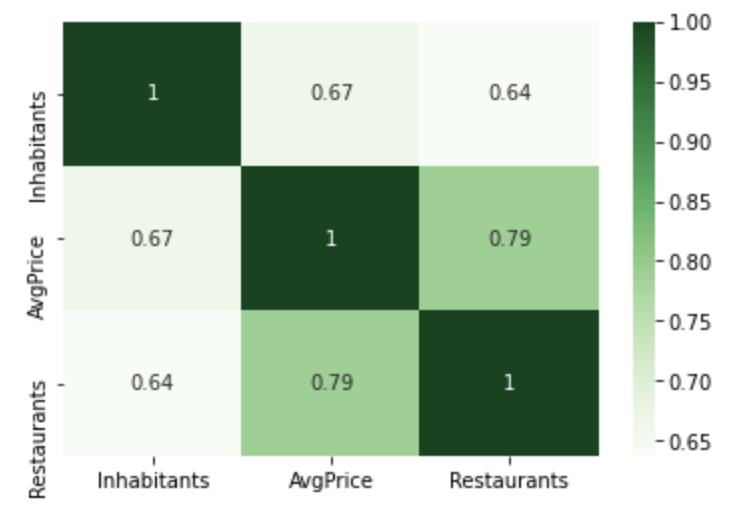
\includegraphics[scale=.4]{CorrMatrixGraph.png} 
		\caption{Graphical representation correlation matrix}
		\label{corrMatrixGraph}
	\end{subfigure}
	\begin{subfigure}{0.5\textwidth}
		\centering
		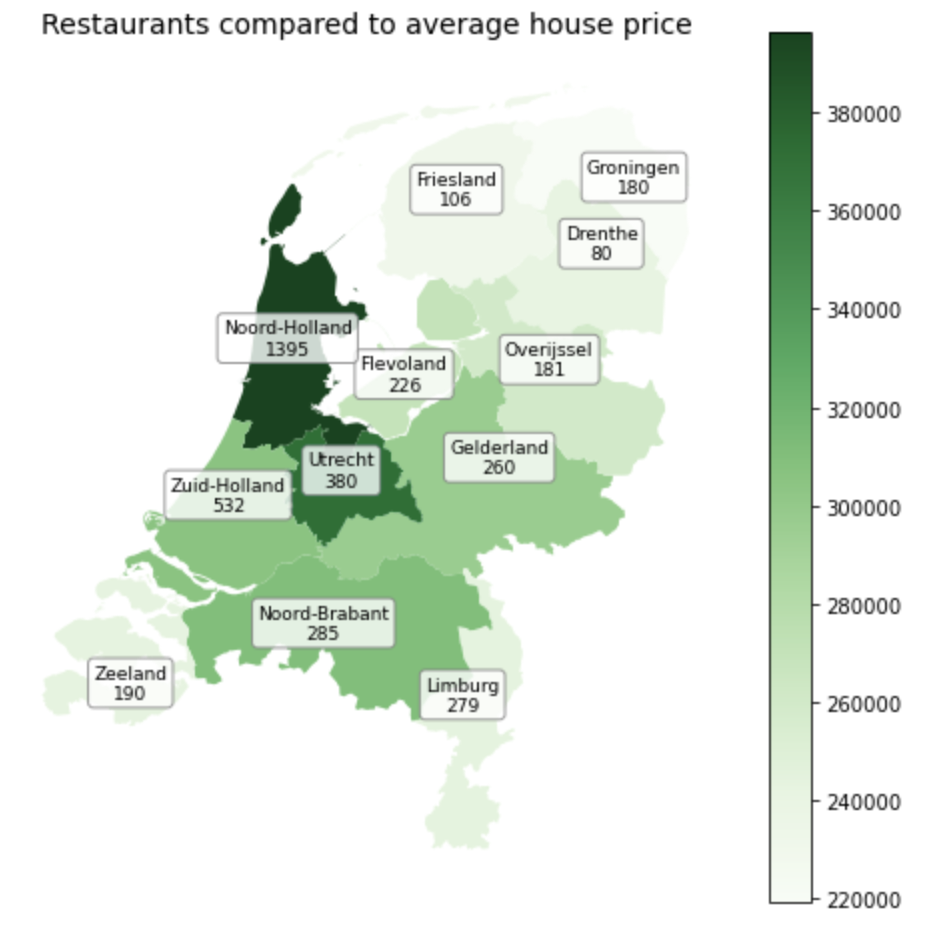
\includegraphics[scale=.4]{Map.png}
		\caption{Colormap of average house price and number of restaurants}
	\end{subfigure}
	\caption{Analysis results}
\end{figure}
\medskip
Looking at the correlation matrix (see figure \ref{corrMatrixGraph}), the number of restaurants in de province capital city has a \textbf{strong} correlation to the average house price in the respective province: the correlation coefficient has a value ≈ .79. This report started with the question if a correlation between the average house price and the number of restaurants exists and the answer based on my analysis is the following:
\medskip
\begin{quote}
\textit{Based on \textbf{FourSquare} data, a statistical strong correlation between the average house price and the number of restaurants in the provinces of the Netherlands exists.}
\end{quote}
\medskip
The main question underlying this report raised another question: does a correlation exists between the number of inhabitants and the average house price? Looking at the correlation matrix, this correlation does exist but is less strong than the number of restaurants (.64 compared to .79). 
\\\\
I think the most important note for this analysis part is that with the right preparation, libraries and add-ons installed, performing an analyses in Python is extremely powerful and easy to execute.